\documentclass[12pt,fleqn]{article}\usepackage{../../common}
\begin{document}
Ders 3

Çapraz çarpımlar hakkında bilinmesi gereken bazı 
şaşırtıcı gelebilecek
kurallar var. Bunlardan bir tanesi $\vec{A} \times \vec{B} \ne \vec{B}
\times \vec{A}$ işlemi. Peki neden böyle? Bunu incelemenin yollarından 
bir 
tanesi 
geometrik olarak düşünmek. Sağ el kuralını 
düşünürsek, yönün neden 
farklı olabileceğini anlarız. İşaretler tam terstir, yani

$$  \vec{A} \times \vec{B} = - \vec{B}\times \vec{A} $$

Determinant açılımını da düşünürsek, ikinci terim 
eksi işareti taşır, ama
çarpım sırası değişince eksi işaretinin yeri değişir. 

Peki $\vec{A} \times \vec{A}$ nedir? Çapraz çarpım alan hesabında 
önemli
olduğuna göre ve $\vec{A} \times \vec{A}$ bir paralelkenar
oluşturamayacağına göre (ya da sıfır alanlı bir 
paralelkenar oluşturacağına
göre) cevap sıfır, daha doğrusu sıfır ``vektörü'' (o 
vektörün büyüklüğü de
tabii ki sıfır).

Uygulamalar

Diyelim ki bize uzayda üç nokta verildi, ve bu noktaları içeren bir 
düzlemin
formülünü bulmamız gerekiyor. Üç nokta, üç boyutlu 
uzayda bir düzlem yaratmak
için yeterli, bunu biliyoruz. Bunun için bir dördüncü nokta $P$ 
hayal
edelim ki bu noktanın öğeleri $x,y,z$ olsun.
\begin{center}
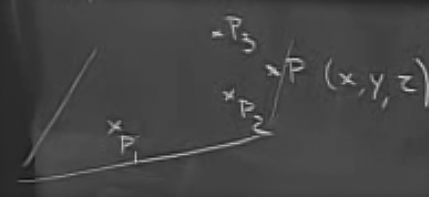
\includegraphics[width=6cm]{3_1.png}
\end{center}
Şimdi düzlemi tanımlayalım. Şu şekilde 3 tane vektör 
yaratalım
\begin{center}
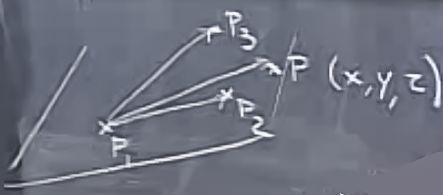
\includegraphics[width=7cm]{3_2.png}
\end{center}
Bu vektörlerin aynı düzlem üzerinde olması, aynı zamanda bu 
vektörlerin
tanımladığı paralelyüz'ün hacimsiz olması demektir. Yani 
birisi
üzerinden bastırıp onu dümdüz etmiştir sanki, sadece alanı 
kalmıştır. 

Bunu matematiksel olarak ifade etmenin yolu şudur:

$$ det(\vec{P_1P},\vec{P_2P},\vec{P_3P}) = 0 $$

Gerçek uygulama bağlamında problem bize $P_1,P_2,P_3$ 
sayılarını vermiş
olurdu.Biz bu sayıları üstteki formüle yerleştirdiğimizde ise 
tanımsız olan
sadece $x,y,z$ kalırdı ve bu $x,y,z$'ler ile beraber elde edilecek 
formül bu
noktaların tanımladığı alan olurdu.

Bu hesabı daha da hızlı yapmanın bir yolu var. Alttaki resmi 
düşünelim. 
\begin{center}
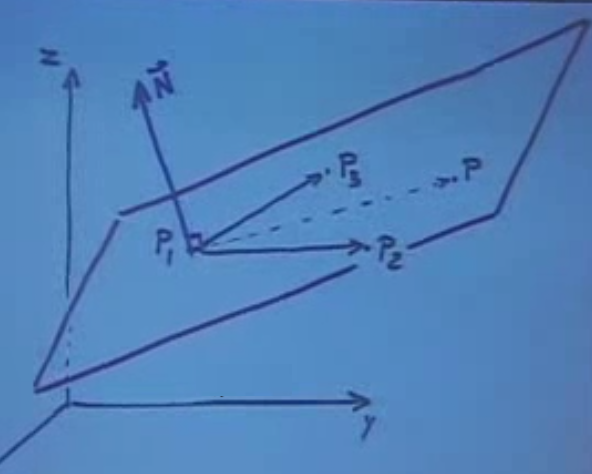
\includegraphics[width=7cm]{3_3.png}
\end{center}
Düzlem üzerindeki iki vektöre dik bir $\vec{N}$'i nasıl
hesaplayacağımızı biliyoruz (çarpraz çarpım ile). 
Ayrıca, $x,y,z$
değişkenlerini içeren üçüncü bir vektör $\vec{P_1P}$'in 
aynı düzlemde
olması demek, bu $\vec{N}$ vektörüne dik olması demektir ($\vec{N}$
``normal vektör'' olarak isimlendirilir). Bunu matematiksel olarak nasıl
ifade ederiz? Dikliğin matematiksel karşılığını biliyoruz, 
noktasal çarpım
sıfır olmalı.

$$ \vec{P_1P} \cdot \vec{N} = 0 $$

$\vec{N}$ hesabı için 

$$ \vec{N} = \vec{P_1P_2} \times \vec{P_1P_3}$$

Bu kadar. 

Ek not, eğer çapraz çarpımın sırasını 
değiştirmiş olsaydım, o zaman üstteki
hesabın ters yönünde bir başka dik vektör elde ederdim, düzlem 
yine aynı
olurdu, sadece başka bir normal vektör olurdu. Bu problem değil, 
herhangi
bir düzlemin sonsuz sayıda normal vektörü olabilir. Elde 
ettiğimiz bir
normal vektörü herhangi bir sabit ile çarpınca yeni bir normal 
vektör elde
etmiş olurum çünkü. 

$$ \vec{P_1P} \cdot \vec{N} = 
\vec{P_1P} \cdot (\vec{P_1P_2} \times \vec{P_1P_3})
$$

Eşitliğin sağındaki çarpıma üçlü çarpım (triple 
product) deniyor. 

Eğer dikkat ettiyseniz, denklemin sağ tarafındaki çapraz 
çarpım işlemine tabi 
tutulan vektörler aynı düzlem içerisinde bulunduğu için, 
çapraz çarpımın sonucu 
bize bulundukları düzleme dik bir vektör verir. Bu vektör, denklemin 
sol 
tarafındaki $\vec{N}$ ile aynı doğrultuda olduğu için bu 
eşitlik her zaman 
sağlanır.


Matrisler

$AB$ şeklindeki bir matris çarpımında herhangi bir hücrenin, 
hangi kolon hangi
satırın noktasal çarpımının sonucu olduğunu hayal edebilmek 
için
alttaki şekil faydalı olabilir. $AB$ çarpımını 
gerçekleştirdikten sonra ortaya 
çıkan matriste, herhangi bir hücreyi ele alalım. Mesela, beşinci 
satır, dördüncü 
kolon. Bu sayı, $A$ matrisinin beşinci satırı ile, $B$ matrisinin 
dordüncü 
kolonunun noktasal çarpımının sonucudur. İşte bu kadar basit.
\begin{center}
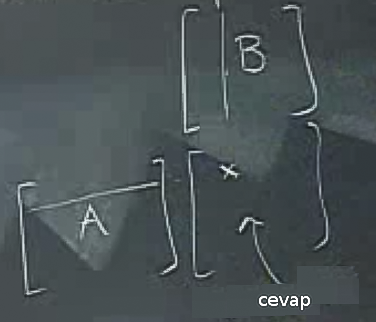
\includegraphics[width=6cm]{3_4.png}
\end{center}
Sezgisel olarak $AB$ çarpımı neyi temsil eder? Bu çarpımı 
şöyle
düşünebiliriz, önce $B$ transformu yap, sonra $A$ transformu yap. Bu 
biraz
acaip gelebilir, çünkü normalde işlemleri soldan sağa yapmaya
alışığızdır. Fakat $AB$'yi belki de sıralı fonksiyon 
işlemleri olarak
görmek daha doğru olur, mesela $f(g(x))$ gibi. Burada önce $g$ 
uygulanır,
sonra $f$ uygulanır. 

$$ (AB)X = A(BX) $$

Üstteki özelliğe birleşim özelliği diyoruz. Bu arada, 
üstteki çarpımın noktasal 
değil, matris çarpımı
olduğuna dikkat edelim. 

Not: $AB \ne BA$. En azından sağdaki çarpımın olabileceğini 
beklemememiz
gerekir. $AB$ çarpımı boyutlar uyduğu için mümkün 
olmuştur, fakat bu uyumlu
boyutlar yerler değişince belki mümkün olmaz. Boyutlar olsa bile 
sonuç
farklı çıkabilir, o sebeple eşitlik farz edilemez. Ufak bir Python 
kodu ile
test edelim:

\begin{minted}[fontsize=\footnotesize]{python}

a = [[2,3,4],[4,4,5],[9,3,2]]
b = [[2,3,9],[4,2,5],[9,3,2]]

print np.dot(a,b)

print np.dot(b,a)
\end{minted}

\begin{verbatim}
[[ 52  24  41]
 [ 69  35  66]
 [ 48  39 100]]
[[97 45 41]
 [61 35 36]
 [48 45 55]]
\end{verbatim}

Sonuçlar farklı çıkacak. 

Örnek

Çevirmek / Rotasyon

Bir düzlem üzerinde bir vektörü $90^o$, saat yönü tersine 
çevirmek için 

$$ R =
\left[\begin{array}{rr}
0 & -1 \\
1 & 0
\end{array}\right]
 $$

İlginç bir durum

$$ R^2 =
\left[\begin{array}{rr}
-1 & 0 \\
0 & -1
\end{array}\right]
 $$

Yani birim matrisinin negatifi. Niye böyle oldu? Düşünelim, eğer
bir vektörü 90 derece döndürürsem, sonra bir daha 90 derece 
döndürürsem, sonuç 
olarak 180 derece döndürmüş olurum, yani tam tersi yöne gitmiş 
olurum. Birim 
matrisin negatifi de budur zaten. 

Matrisler denklem sistemlerini temsil edebilirler, alttaki gibi
\begin{center}
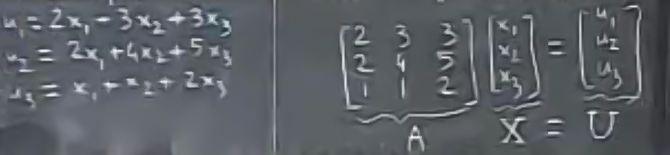
\includegraphics[width=14.9cm]{3_5.png}
\end{center}
Bu tür sistemlerde belki $X$ değerleri verilmiştir, $U$'yu 
hesaplamamız
isteniyordur, ya da tam tersi de olabilir, $U$ verilmiştir, $X$
hesaplamamız isteniyordur. Ters yönde gitmek için matris tersini 
(inverse)
almak gerekir.

Not: Bir matrisin tersini alabilmemiz için onun kare matrisi olması 
gerekir,
yani boyutu $n$ x $n$ olmalıdır. 

Ters yönde çözüme gelelim. Mesela elimizde şöyle bir sistem 
var

$$  AX = B$$

$$  A^{-1}(AX) = A^{-1}B$$

$$  X = A^{-1}B$$

Böylece $X$'i elde edebilmiş oluruz. O zaman $A$ matrisinin tersini alma
operasyonunu yapabiliyorsak, istediğimiz herhangi bir lineer denklem
sistemini çözebiliriz demektir. 

Aşağıdaki eşitlik de bir matrisin tersini bulabilmek adına 
geçerlidir. 

$$ A^{-1} = \frac{1}{det(A)}  = adj(A)$$

Üstte $adj$ diye tanımlanan bir matrisin bitişiğini (adjoint matrix) 
nasıl
buluruz?

Mesela

$$ 
\left[\begin{array}{rrr}
2 & 3 & 3 \\
2 & 4 & 5 \\
1 & 1 & 2
\end{array}\right]
 $$

Adımlar:

1) Bu matrisin ``minörlerini'' bulmak lazım. O nedir? Aslında 
minörleri
determinant işlemini işlediğimizde görmüştük, sadece bu 
ismi vermemiştik.
Onlar en üst satırdaki matris hücrelerini teker teker merkez alıp, 
onun
satırını, kolonunu iptal ettikten sonra geri kalan daha ufak 
bölgenin
determinantlarıydı. Bitişiklik için bu hesabı sadece üst 
satır için değil,
tüm hücreler için yapacağız. Üstteki örnek için

$$ 
\left[\begin{array}{rrr}
3 & -1 & -2 \\
3 & 1 & -1 \\
3 & 4 & 2
\end{array}\right]
 $$




2) Katsayıları bulma işlemi. Determinant işlemini bir matrisin 
minörlerini 
toplayarak buluyoruz. Ve her minörün önüne şimdi 
göstereceğimiz kurala göre "+" 
veya "-" işareti geliyor. Katsayı kuralımızın formülü şu 
şekildedir 
$(-1)^{m+n}$. Bu formülde "m" satır numarası, "n" ise kolon 
numarasıdır. Formülü 
daha iyi kavrayabilmek adına dama tahtası gibi bir şekil 
düşünelim, bunun
üzerinde +,- işaretleri olsun. 

$$ 
\begin{array}{rr}
+ - + - + \\
- + - + - \\
+ - + - + \\
- + - + - \\
\end{array}
 $$


Örnekteki bitişiklik ise şu hale gelir:

$$ 
\left[\begin{array}{rrr}
3 & 1 & -2 \\
-3 & 1 & 1 \\
3 & -4 & 2
\end{array}\right]
 $$

3) Devriğini Al (Transpose)

Satırlar ve kolonların yerini değiştir. 

$$ 
\left[\begin{array}{rrr}
3 & -3 & 3 \\
1 & 1 & -4 \\
-2 & 1 & 2
\end{array}\right]
 $$

4) Her şeyi $det(A)$'ya böl 

$$ 
\left|\begin{array}{rrr}
2 & 3 & 3 \\
2 & 4 & 5 \\
1 & 1 & 2
\end{array}\right| = 3
 $$

$$ A^{-1} = 
\frac{1}{3}
\left[\begin{array}{rrr}
3 & -3 & 3 \\
1 & 1 & -4 \\
-2 & 1 & 2
\end{array}\right]
 $$

\end{document}



